\documentclass[fontset=windows]{article}
\usepackage[margin=1in]{geometry}%设置边距,符合Word设定
\usepackage[UTF8]{ctex}
\usepackage{setspace}
\usepackage{amsmath}
\usepackage{amssymb}
\numberwithin{figure}{section}
\usepackage{array}
\usepackage{lipsum}
\usepackage{float}
\usepackage{graphicx}%插入图片
\usepackage[dvipsnames]{xcolor}
\usepackage{authblk}
\usepackage{algorithm,algorithmic}
\usepackage{listings,matlab-prettifier}
\lstset{
	language=matlab, % 设置代码语言为Matlab
    basicstyle=\ttfamily, % 设置字体为等宽字体
    numbers=left, % 行号在左边显示
    numberstyle=\tiny, % 设置行号字体大小
    stepnumber=1, % 行号递增步长
    numbersep=5pt, % 行号到代码的距离
    backgroundcolor=\color{gray!10}, % 设置代码的背景颜色
    showspaces=false,
    showstringspaces=false,
    showtabs=false,
    frame=single, % 设置代码框
    rulecolor=\color{black},
    tabsize=2,
    breaklines=true,
    breakatwhitespace=true,
    title=\lstname,
	keywordstyle=\bfseries\color{NavyBlue},
	morekeywords={var,};
	emphstyle=\bfseries\color{Rhodamine}, % 强调词样式设置
    commentstyle=\itshape\color{black!50!white}, % 设置注释样式,斜体,浅灰色
    stringstyle=\bfseries\color{PineGreen!90!black}, % 设置字符串样式
	columns=flexible,}
\graphicspath{{Figures8/}}%文章所用图片在当前目录下的 Figures目录

\usepackage{hyperref} % 对目录生成链接,注:该宏包可能与其他宏包冲突,故放在所有引用的宏包之后
\hypersetup{colorlinks = true,  % 将链接文字带颜色
	linkcolor=black, % 将链接文字黑色
	bookmarksopen = true, % 展开书签
	bookmarksnumbered = true, % 书签带章节编号
	} % 作者
\bibliographystyle{plain}% 参考文献引用格式

\renewcommand{\contentsname}{\centerline{目录}} %经过设置word格式后,将目录标题居中

\title{\heiti\zihao{2} 《统计信号处理》第八教学单元研讨题}
\author{杨 鼎,韦可雷,高司博,高涵博}
\date{}

\begin{document}
\maketitle
\thispagestyle{empty}

%\begin{abstract}
%	\lipsum[2]
%\end{abstract}

%\tableofcontents
%\setcounter{page}{0}
%\newpage

\section{研讨题1}
考虑WGN中二元假设检验问题

\begin{align*}
    \begin{matrix}
        \mathcal{H}_0: & z[k]=n[k]      \\
        \mathcal{H}_1: & z[k]=s[k]+n[k]
    \end{matrix}\quad k=0,1,\ldots,N-1
\end{align*}
噪声是服从\(n(k)\sim \mathcal{N}(0,\sigma^2)\)的WGN。

\subsection*{(1)若\(s[k]=A,A\)未知,确定当\(\sigma^2\)已知和未知时的GLRT的渐进性能。}

当\(\sigma^2\)已知时,GLRT计算可以参考课本例6.2与例6.4。

A的最大似然估计为:
\begin{align*}
    \hat{A}=\overline{z}=\frac{1}{N}\sum_{k=0}^{N-1}z(k)
\end{align*}
利用GLRT,我们有
\begin{align*}
    L_G(\mathbf{z})
    =\frac{p(\mathbf{x};A,\mathcal{H}_1)}{p(\mathbf{z};\mathcal{H}_0)}
    =\frac{(2\pi \sigma^2)^{-N/2}\exp\left[-\frac{1}{2\sigma^2}\sum_{n=0}^{N-1}(z[n]-\overline{z})^2\right]}
    {(2\pi \sigma^2)^{-N/2}\exp\left[-\frac{1}{2\sigma^2}\sum_{n=0}^{N-1}z^2[n]\right]}
    \begin{matrix}
        \mathcal{H}_1 \\>\\<\\\mathcal{H_0}
    \end{matrix}\gamma
\end{align*}
取对数化简有:
\begin{align*}
    \ln L_G(\mathbf{z})
     & =-\frac{1}{2\sigma^2}\left(\sum_{n=0}^{N-1}z^2[n]-
    2\overline{z}\sum_{n=0}^{N-1}z[n]+n\overline{z}^2-\sum_{n=0}^{N-1}z^2[n]\right)             \\
     & =-\frac{1}{2\sigma^2}(-2N\overline{z}^2+N\overline{z})=\frac{N\overline{z}^2}{2\sigma^2}
    \begin{matrix}
        \mathcal{H}_1 \\>\\<\\\mathcal{H_0}
    \end{matrix}\gamma
\end{align*}
判决条件可以写为
\begin{align*}
    \vert \overline{z}\vert >\gamma
\end{align*}
检验统计量的渐进分布为
\begin{align*}
    2\ln L_G(\mathbf{z})=\frac{N\overline{z}^2}{2\sigma^2}\overset{a}{\sim}
    \left\{\begin{matrix}
               \chi^2_1                   & \mathcal{H}_0 \\
               \chi_1^{\prime 2}(\lambda) & \mathcal{H}_1
           \end{matrix}
    \right.
\end{align*}
其中\(\lambda=\frac{NA^2}{\sigma^2}\),因此对于这种特殊情况,有限数据记录渐进PDF是精确成立的:
\begin{align*}
    \frac{\overline{z}}{\sigma/\sqrt{N}}\sim
    \left\{\begin{matrix}
               \mathcal{N}(0,1)                        & \mathcal{H}_0 \\
               \mathcal{N}(\frac{\sqrt{N}A}{\sigma},1) & \mathcal{H}_1
           \end{matrix}
    \right.
\end{align*}
NP准则确定虚警率与门限的关系为
\begin{align*}
    P_{FA}=2Q\left(\frac{\gamma^{\prime}}{\sqrt{\sigma^2/N}}\right)
\end{align*}
检测概率为
\begin{align*}
    P_D=Q\left[Q^{-1}\left(\frac{P_{FA}}{2}\right)-\sqrt{\frac{NA^2}{\sigma^2}}\right]+
    Q\left[Q^{-1}\left(\frac{P_{FA}}{2}\right)+\sqrt{\frac{NA^2}{\sigma^2}}\right]
\end{align*}

\subsection*{(2)若\(s[k]\sim A,A\)未知但已知其取值为-1或1,\(\sigma^2\)未知,求解GLRT判决式并分析是否CFAR。}

当\(\sigma^2\)未知时,GLRT的计算参考教材例6.5,等效检验统计量为【】

其PDF并不依赖于\(\sigma^2\),检测性能要比\(\sigma^2\)已知时的检测性能稍差,但在N足够大时,性能衰减是相当小的,基本与\(\sigma^2\)已知时的特性相同,一下是GLRT理论渐进性能与实际渐进性能的比较:

设置信噪比\(\lambda=\frac{NA^2}{\sigma^2}=5,\sigma^2=1\),对于\(N=10,A=\sqrt{\frac{\lambda\sigma^2}{N}}=\sqrt{2}/2\),而对于\(N=30,A=\sqrt{\frac{\lambda\sigma^2}{N}}=\sqrt{6}/6\)。给定虚警概率,分别由理论计算式与蒙特卡洛仿真计算得到的对应检测概率,如图所示

【图】

可见N值越大,GLRT渐进性能越好,N=30时,实际值与理论值十分逼近。

当\(\sigma^2\)未知时,由例9.1可知,\(\sigma^2_0\)和\(\sigma^2_1\)的极大似然估计为
\begin{align*}
    \sigma^2_0 & =\frac{1}{N}\sum_{k=0}^{N-1}z^2[k]           \\
    \sigma^2_1 & =\frac{1}{N}\sum_{k=0}^{N-1}(z[k]-\hat{A})^2
\end{align*}
A的最大似然估计为:
\begin{align*}
    \hat{A}=sgn(\overline{z})
\end{align*}

同1的推导过程
\begin{align*}
    L_G(\mathbf{z})
     & =\frac{p(\mathbf{z};\hat{A},\hat{\sigma}^2_1,\mathcal{H}_1)}{p(\mathbf{z};\hat{\sigma}^2_0,\mathcal{H}_0)}
    =\frac{(2\pi \hat{\sigma}^2)^{-N/2}\exp\left[-\frac{1}{2\hat{\sigma}^2}\sum_{k=0}^{N-1}(z[k]-sgn(\overline{z}))^2\right]}
    {(2\pi \hat{\sigma}_0^2)^{-N/2}\exp\left[-\frac{1}{2\hat{\sigma}_0^2}\sum_{k=0}^{N-1}z^2[k]\right]}           \\
     & =\frac{(2\pi \hat{\sigma}^2)^{-N/2}\exp\left(-\frac{N}{2}\right)}
    {(2\pi \hat{\sigma}_0^2)^{-N/2}\exp\left(-\frac{N}{2}\right)}=\left(\frac{\hat{\sigma}_0^2}{\hat{\sigma}_1^2}\right)^{N/2}
    \begin{matrix}
        \mathcal{H}_1 \\>\\<\\\mathcal{H_0}
    \end{matrix}\gamma
\end{align*}

令\(n[k]=\sigma u[k]\),其中\(u[k]\)是方差为1的WGN。在\(\mathcal{H}_0\)条件下,由于\(z[k]=n[k]\),等效检验统计量为
\begin{align*}
    T(\mathbf{z})
     & =\frac{\overline{z}^2}{\hat{\sigma}^2_1}
    =\frac{\frac{1}{N}\sum_{k=0}^{N-1}z^2[k]}{\frac{1}{N}\sum_{k=0}^{N-1}(z[k]-\hat{A})^2}       \\
     & =\frac{\frac{1}{N}\sum_{k=0}^{N-1}\sigma^2u^2[k]}
    {\frac{1}{N}\sum_{k=0}^{N-1}(\sigma u[k]-sgn(\sigma \overline{u}))^2}                        \\
     & =\frac{\sum_{k=0}^{N-1}\sigma^2u^2[k]}{\sum_{k=0}^{N-1}(\sigma u[k]-sgn(\overline{u}))^2}
\end{align*}
其中PDF依赖于\(\sigma^2\),含有未知参数,因此不是CFAR检测器。

\subsection*{(3)若\(s[k]=A(-1)^k\),其中A未知,噪声方差\(\sigma^2\)未知,求解GLRT判决式并分析渐进性能。}

与第一问不同之处在于A的最大似然估计形式发生了变化:
\begin{align*}
    \hat{A}=\frac{1}{N}\sum_{k=0}^{N-1}(-1)^kz(k)
\end{align*}
由此,\(\sigma^2_0\)和\(\sigma^2_1\)的最大似然估计也变为
\begin{align*}
    \sigma^2_0 & =\frac{1}{N}\sum_{k=0}^{N-1}z^2[k]                 \\
    \sigma^2_1 & =\frac{1}{N}\sum_{k=0}^{N-1}(z[k]-(-1)^k\hat{A})^2
\end{align*}
其他求解过程同第一问,由于\(\lambda=\frac{NA^2}{\sigma^2}\),其检测概率计算式以及虚警概率计算式均不变,以下是GLRT理论渐进性能与实际渐进性能的比较。


综上,当N值越大,GLRT渐进性能约逼近理论值,且与第一问渐进性能相似。

\section{研讨题2:}
考虑二元假设检验问题

\begin{align*}
    \begin{matrix}
        H_0: & z(k)=n(k)   \\
        H_1: & z(k)=A+n(k)
    \end{matrix}\quad k=0,1,\cdots N-1
\end{align*}
其中A已知且\(A>0,n[k]\)为PDF为\(p(n[k])\)的IID样本,其均值为零,方差为\(\sigma^2\)。若\(\mathcal{H}_1\)判决式为\(T(\mathbf{z})=\frac{1}{N}\sum_{k=0}^{N-1}z[k]>\gamma\)。

\subsection*{(1)应用中心极限定理求解\(P_{FA}\)和\(P_D\),分析在均值和方差不变的情况下,\(p(n[k])\)对于性能有何影响?}


\subsection*{(2)若n[k]服从拉普拉斯PDF,其性能相比于高斯噪声如何?}

\newpage
\section{研讨题3:非高斯噪声的模拟与分析}

\subsection*{(1)采用反函数法生成教材(10.1)式的拉普拉斯分布,并根据统计分析超过3\(\sigma\)的概率。}

教材(10.1)式的拉普拉斯分布为
\begin{align*}
    p(w[n])=\frac{1}{\sqrt{2\sigma^2}}\exp\left(-\sqrt{\frac{2}{\sigma^2}}\vert w[n]\vert\right)\quad -\infty<w[n]<\infty
\end{align*}
其累积分布函数(CDF)为
\begin{align*}
    F(w[n]) & =\left\{\begin{matrix}
                          \frac{1}{2}\exp(\sqrt{\frac{2}{\sigma^2}}w[n])    & w[n]<0         \\
                          1-\frac{1}{2}\exp(-\sqrt{\frac{2}{\sigma^2}}w[n]) & w[n]\geqslant0 \\
                      \end{matrix} \right. \\
            & =\frac{1}{2}\left[1+sgn(w[n])(1-\exp\left(-\sqrt{\frac{2}{\sigma^2}}\vert w[n]\vert\right))\right]
\end{align*}
其中\(sgn(\cdot)\)为符号函数,当\(w[n]>0\)时,\(sgn(w[n])=1\),当\(w[n]<0\)时,\(sgn(w[n])=-1\)。可以解得逆函数为
\begin{align*}
    F^{-1}(u)=-\frac{\sigma}{\sqrt{2}}sgn(u-0.5)\ln(1-2\vert u-0.5\vert)
\end{align*}
其中\(u\sim \mathcal{N}(0,1)\)。因此可以利用均匀分布生成拉普拉斯分布。算法如下

\begin{algorithm}[H]
    \caption{Laplace Distribution}
    \label{Laplace}
    \begin{algorithmic}[1]
        \REQUIRE \(\sigma\);
        \ENSURE \(w[n]\);
        \STATE \(U\sim \mathcal{U}(0,1)\)
        \IF {\(U>0.5\)}
        \STATE \(P=2*U\)
        \STATE \(w[n]=-\sqrt{\frac{\sigma^2}{2}}\ln(2-P)\)
        \ELSE
        \STATE \(P=2*(1-U)\)
        \STATE \(w[n]=\sqrt{\frac{\sigma^2}{2}}\ln(P)\)
        \ENDIF
        \STATE \textbf{return} \(w[n]\)
    \end{algorithmic}
\end{algorithm}

利用MATLAB编程模拟,产生数据长度N=5000时的w[n],比较拉普拉斯分布概率密度函数与生成w[n]数据的分布如图\ref*{fig:1}。设定\(\sigma=1\),图中红色曲线为拉普拉斯概率密度函数,蓝色柱状图为反函数法生成的服从拉普拉斯分布的数据w[n]的分布图图中可以发现反函数法生成数据近似服从拉普拉斯分布。

\begin{figure}[H]
    \centering
    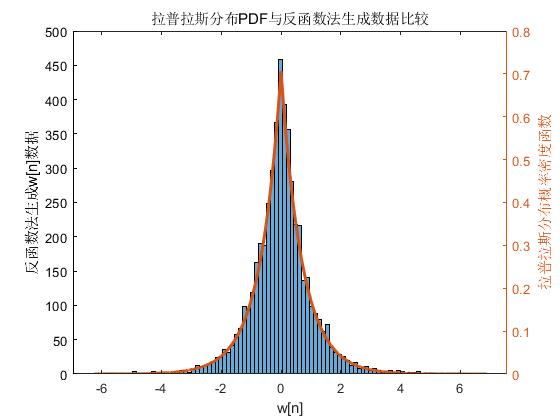
\includegraphics[scale=0.5]{1.jpg}
    \caption{拉普拉斯分布概率密度函数与反函数法生成w[n]数据比较图}
    \label{fig:1}
\end{figure}

样本超过\(3\sigma\)的概率
\begin{align*}
    P\{\vert w[n]\vert >3\sigma\}
     & =2P\{w[n]<-3\sigma\} \\
     & =2F(-3\sigma)        \\
     & =\exp(-3\sqrt{2})    \\
     & =0.0144
\end{align*}

图\ref*{fig:2}显示了随着样本数N的增大,数据超过\(3\sigma\)的概率变化曲线。可以看到随着样本数N的增加,数据超过\(3\sigma\)的概率逐渐趋于理论值\(\exp(-3\sqrt{2})\)
\begin{figure}[H]
    \centering
    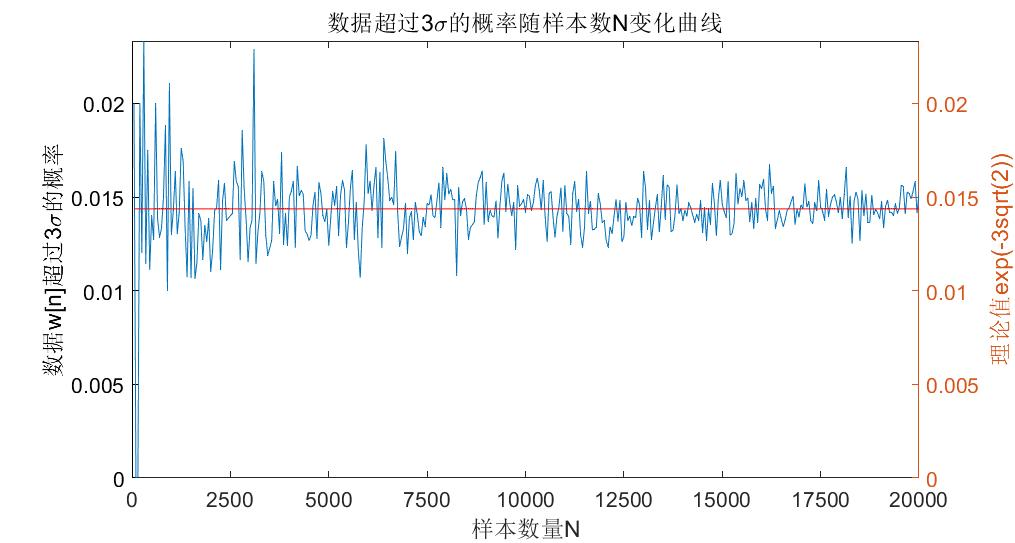
\includegraphics[scale=0.35]{2.jpg}
    \caption{数据超过\(3\sigma\)的概率随数据长度的变化曲线图}
    \label{fig:2}
\end{figure}

\subsection*{(2)模拟下式的混合高斯PDF,假定\(\sigma^2_2>\sigma^2_1\)。假定混合高斯平均功率\(\sigma^2\)为1,\(\varepsilon=0.01\),根据不同\(\sigma^2_2,\sigma^2_1\)数值下样本统计分析超过3\(\sigma\)的概率。}
\begin{align*}
    p(n)=(1-\varepsilon)\frac{1}{\sqrt{2\pi \sigma^2_1}}\exp\left(-\frac{n^2}{2\sigma^2_1}\right)+
    \varepsilon \frac{1}{\sqrt{2\pi \sigma^2_2}}\exp\left(-\frac{n^2}{2\sigma^2_2}\right)
\end{align*}

已知混合高斯分布平均功率\(\sigma^2=1\),则\((1-\varepsilon)\sigma^2_1+\varepsilon\sigma^2_2=\sigma^2=1\),所以\(\sigma^2_1=\frac{1-\varepsilon\sigma^2_2}{1-\varepsilon}\),由\(\sigma^2_2>\sigma^2_1\),解得\(\sigma^2_2>1,\sigma^2_1<1\)。

\textbf{1}.首先考虑生成符合高斯分布的随机变量。由于高斯分布的累积分布函数(CDF)\(\Phi(x)\)不是初等函数,它的逆函数无法用解析形式表示,因此高斯分布的随机变量无法用逆变换法产生,但是可以通过Box-Muller变换法产生。

Box-Muller变换法与逆变换法有关。考虑同时构造两个独立的高斯分布的随机变量:随机变量X和Y相互独立,且均服从正态分布,其联合概率密度函数为
\begin{align*}
    f(x,y)
     & =\frac{1}{\sqrt{2\pi \sigma^2_1}}\exp(-\frac{x}{2\sigma^2_1})\cdot
    \frac{1}{\sqrt{2\pi\sigma^2_1}}\exp(-\frac{y}{2\sigma^2_1})           \\
     & =\frac{1}{2\pi \sigma^2_1}\exp(-\frac{x^2+y^2}{2\sigma^2_1})
\end{align*}
这个联合概率密度分布的累积分布函数很容易计算,它的积分\(I^2\)是
\begin{align*}
    I^2
     & =\int \int_{\Omega}\frac{1}{2\pi \sigma^2_1}\exp(-\frac{x^2+y^2}{2\sigma^2_1})dxdy   \\
     & =\frac{1}{2\pi \sigma^2_1}\int \int_{\Omega}\exp(-\frac{r^2}{2\sigma^2_1})rdrd\theta \\
     & =\int_{0}^{2\pi}\frac{1}{2\pi}d\theta \cdot
    \int_{0}^{+\infty}\frac{1}{\sigma^2_1}\exp(-\frac{r^2}{2\sigma^2_1})rdr
\end{align*}
积分计算过程中进行了一次从直角坐标系到极坐标系的变换,关于\(\theta\)和r的累积分布函数很容易计算
\begin{align*}
    F_R        & =1-\exp(-\frac{r^2}{2\sigma^2_1}),r\in [0,\infty) \\
    F_{\Theta} & =\frac{\theta}{2\pi },\theta\in [0,2\pi)
\end{align*}

利用逆变换方法,这两个变量\(\Theta\)和\(R\)可以通过两个独立的随机变量\(U_1\sim \mathcal{U}(0,1)\)和\(U_2\sim \mathcal{U}(0,1)\)构造出来

\begin{align*}
    R      & =\sigma_1\sqrt{-2\ln(U_1)} \\
    \Theta & =2\pi U_2
\end{align*}

根据极坐标系到直角坐标系的变换关系
\begin{align*}
    X & =R\cos(\Theta) \\
    Y & =R\sin(\Theta)
\end{align*}
可以得到
\begin{align*}
    X & =\sigma_1\sqrt{-2\ln U_1}\cos(2\pi U_2) \\
    Y & =\sigma_1\sqrt{-2\ln U_1}\sin(2\pi U_2)
\end{align*}
任取X或Y均服从\(\mathcal{N}(0,\sigma^2_1)\)。

同理,若\(U_1^{\prime}\sim \mathcal{U}(0,1),U_2^{\prime}\sim \mathcal{U}(0,1)\),则可以构造出
\begin{align*}
    X^{\prime} & =\sigma_2\sqrt{-2\ln U_1^{\prime}}\cos(2\pi U_2^{\prime}) \\
    Y^{\prime} & =\sigma_2\sqrt{-2\ln U_1^{\prime}}\sin(2\pi U_1^{\prime})
\end{align*}
任取\(X^{\prime}\)或\(Y^{\prime}\)均服从\(\mathcal{N}(0,\sigma^2_2)\)。

\textbf{2}.其次考虑由两个高斯分布的随机变量生成服从混合高斯分布的随机变量。已知混合高斯分布的混合系数分别为\(1-\varepsilon=0.99\)和\(\varepsilon=0.01\),可以从服从\(\mathcal{N}(0,\sigma^2_1)\)和\(\mathcal{N}(0,\sigma^2_2)\)的两个随机变量中以概率0.99和0.01随机选取,就可以得到要求的混合高斯分布。

生成要求的混合高斯分布的算法如下
\begin{algorithm}[H]
    \caption{Gaussian Mixture}
    \label{alg:GMM}
    \begin{algorithmic}[1]
        \REQUIRE \(\sigma_1\ and\ \varepsilon(\varepsilon\in [0,1],\sigma^2_1\in (0,\frac{1}{\varepsilon^2+(1-\varepsilon)^2}))\);
        \ENSURE \(n\);
        \STATE \(U_i\overset{i.i.d}{\sim} \mathcal{U}(0,1),i=1,2,\cdots,5\)
        \STATE \(n_1=\sigma_1\sqrt{-2\ln U_1}\cos(2\pi U_2)\)
        \STATE \(\sigma_2=\frac{1-(1-\varepsilon)\sigma^2_1}{\varepsilon},n_2=\sigma_2\sqrt{-2\ln U_3}\cos(2\pi U_4)\)
        \IF {\(U_5>\varepsilon\)}
        \STATE \(n=n_2\)
        \ELSE
        \STATE \(n=n_1\)
        \ENDIF
        \STATE \textbf{return} \(n\)
    \end{algorithmic}
\end{algorithm}

利用MATLAB编程实现算法\ref*{alg:GMM},得到图\ref*{fig:3}。由于\(\varepsilon=0.01\)时混合高斯分布与单个高斯分布十分相近,难以分辨,所以图\ref*{fig:3}中\(\varepsilon=0.5,\sigma_1^2=0.5,\sigma^2_2=7/4\),数据n长度N为2000。图中直方图代表利用变换法生成的数据n的分布,红色实线代表对应的混合高斯分布的概率密度函数,可以看出生成的数据近似符合混合高斯分布。图中也画出了组成混合高斯分布的单个高斯分布的概率密度函数作为比较,分别为蓝色虚线和绿色虚线。可以求出数据的方差为\(0.9804\approx1\),说明生成的数据符合要求。

\begin{figure}[H]
    \centering
    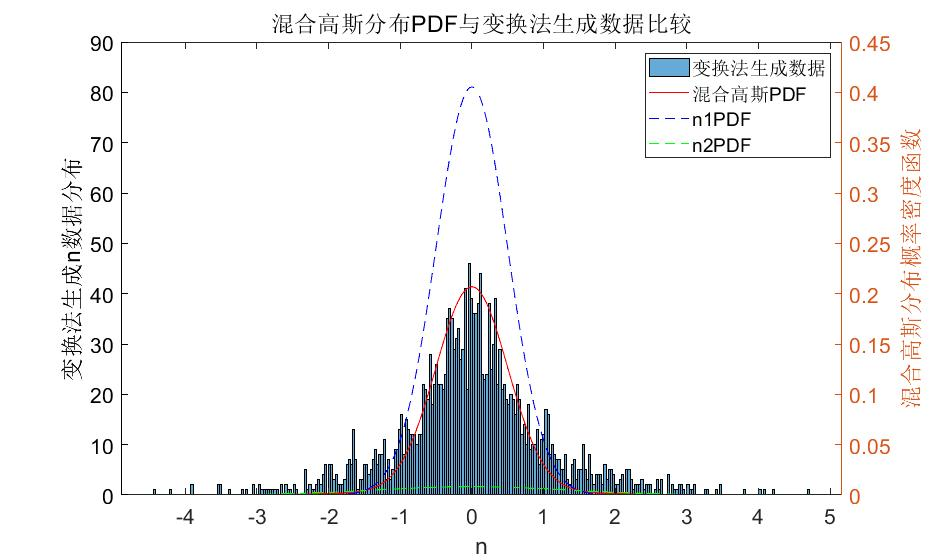
\includegraphics[scale=0.4]{5.jpg}
    \caption{变换法生成数据分布与混合高斯分布比较图}
    \label{fig:3}
\end{figure}

根据算法\ref*{alg:GMM}可以发现,混合高斯分布可以等效为多个高斯分布的加权平均
\begin{align*}
    p(n)=p(n|k=1)P\{k=1\}+p(n|k=2)P\{k=2\}
\end{align*}
其中
\begin{align*}
    P\{k=1\} & =1-\varepsilon                                                             \\
    p(n|k=1) & =\frac{1}{\sqrt{2\pi \sigma^2_1}}\exp\left(-\frac{n^2}{2\sigma^2_1}\right) \\
    P\{k=2\} & =\varepsilon                                                               \\
    p(n|k=2) & =\frac{1}{\sqrt{2\pi \sigma^2_2}}\exp\left(-\frac{n^2}{2\sigma^2_2}\right) \\
\end{align*}
所以混合高斯分布样本超过\(3\sigma\)的概率为多个高斯分布样本超过\(3\sigma\)的概率的加权平均,即
\begin{align*}
    P\{\vert n\vert>3\sigma\}
     & =P\{k=1\}P\{\vert n_1\vert>3\sigma\}+P\{k=2\}P\{\vert n_2\vert>3\sigma\}                                              \\
     & =2(1-\varepsilon)\Phi(-\frac{3\sigma}{\sigma_1})+2\varepsilon \Phi(-\frac{3\sigma}{\sigma_2})                         \\
     & =2(1-\varepsilon)\Phi(-3\sqrt{\frac{(1-\varepsilon)}{1-\varepsilon\sigma_2^2}})+2\varepsilon\Phi(-\frac{3}{\sigma_2})
\end{align*}
其中\(\Phi(x)\)为标准正态分布的累积分布函数。

图\ref*{fig:4}显示了\(\varepsilon=0.01\)时,样本超过\(3\sigma\)的概率随\(\sigma^2_2\)的变化曲线,随着\(\sigma^2_2\)的增长,概率逐渐趋于稳定。

\begin{figure}[H]
    \centering
    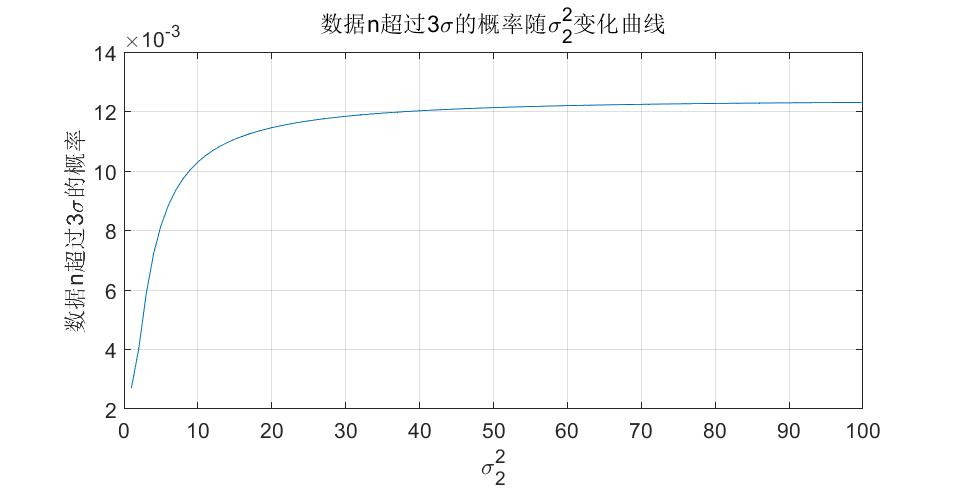
\includegraphics[scale=0.4]{4.jpg}
    \caption{数据超过\(3\sigma\)的概率随\(\sigma^2_2\)的变化曲线图}
    \label{fig:4}
\end{figure}

图\ref*{fig:5}显示了\(\varepsilon=0.01\)时,随着数据长度N的变化,数据超过\(3\sigma\)的概率的变化曲线,这时\(\sigma_1=0.5,\sigma_2=8.6747\),可以发现随着数据长度增长,概率趋于理论值0.0073。

\begin{figure}[H]
    \centering
    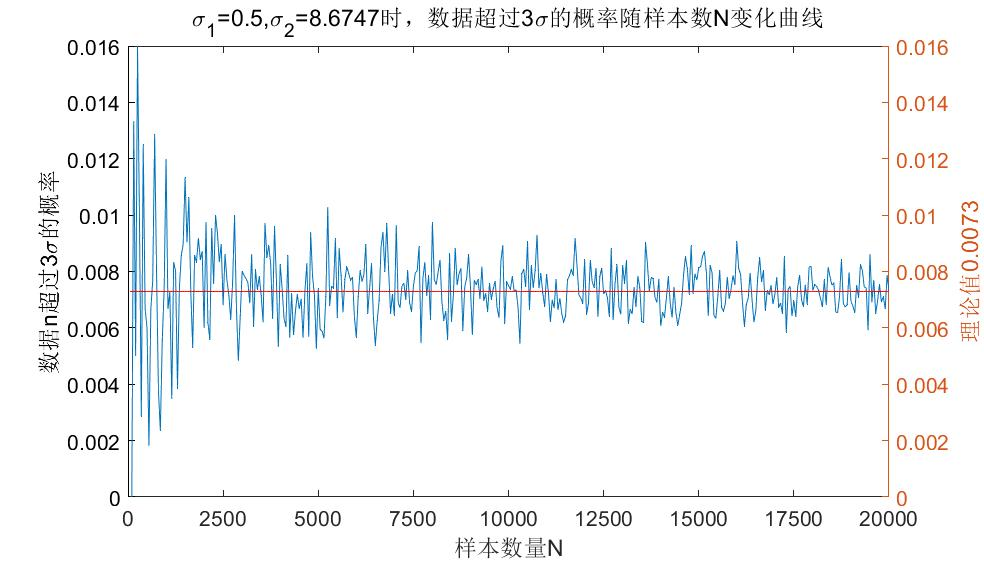
\includegraphics[scale=0.4]{3.jpg}
    \caption{数据超过\(3\sigma\)的概率随数据长度N的变化曲线图}
    \label{fig:5}
\end{figure}



\bibliography{books}
\end{document}